%!TEX root = ./icml2016.tex

\section{Related Work}

\begin{figure}[t]
	\centering
	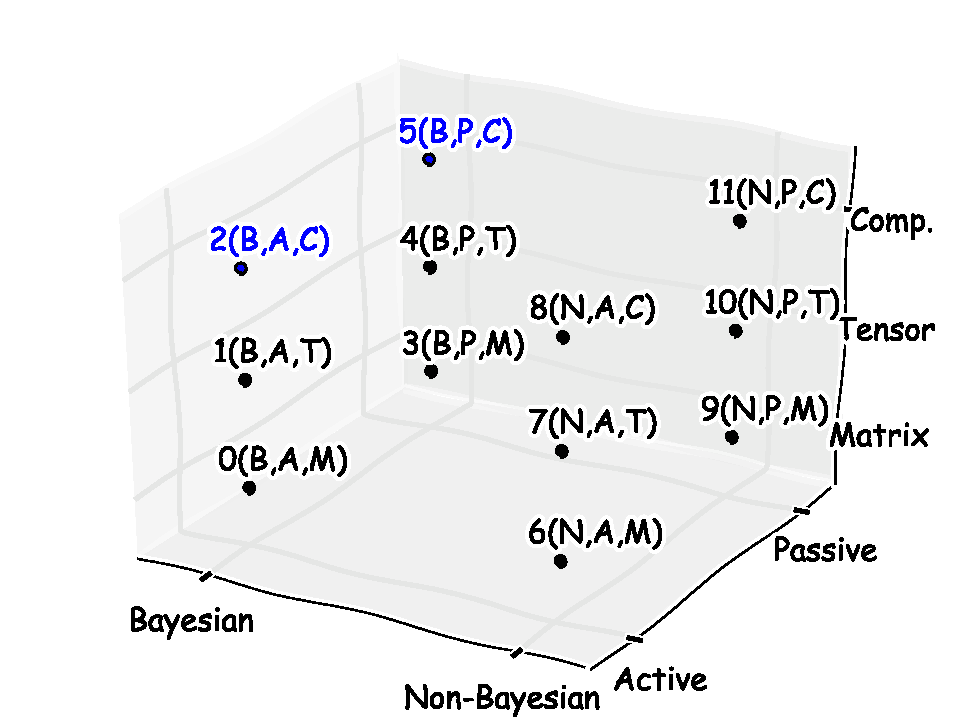
\includegraphics[width=\linewidth]{images/3d_plot.pdf}			
	\caption{\label{fig:related3d}Scope of our work}
\end{figure}

\begin{itemize}
\item [B,A,M] Efficient Thompson Sampling for OnlineMatrix-Factorization Recommendation\cite{kawale2015efficient}. Active learning and search on low-rank matrices \cite{sutherland2013active}. Collaborative filtering as multi armed bandit \cite{guillou2015collaborative}
\item [N,A,M] Matrix completion with queries \cite{ruchansky2015matrix}.
\item [B,P,M] PMF \cite{mnih2007probabilistic} ...
\item [N,P,M] NMF\cite{lee1999learning} ...
\item [B,P,T] Bayesian Tensor Factorisation models. CANDECOMP/PARAFAC (CP) decomposition \cite{xiong2010temporal,schmidt2009probabilistic}, CP and TUCKER3 \cite{yilmaz2012algorithms}
\item [N,A,T] Populating knowledge graph with active learning (IBM) \cite{kajino2015active}
\item [N,P,T] Rescal \cite{nickel2011three}, TransE \cite{bordes2013translating}, and many others.
\item [N,P,C] Compositional vector space model \cite{Neelakantan2015}, 
\end{itemize}

Might be relevant, but not positioned in the figure.
\begin{itemize}
\item Clustering based Bayesian approach for learning relations: Infinite relational model based on entity clustering \cite{kemp2006learning}.
\item Path ranking algorithm (graph feature model) \cite{Lao2010}
\end{itemize}
